\appendix

\setcounter{figure}{0}
\setcounter{table}{0}
\setcounter{section}{0}
\renewcommand{\theequation}{\Alph{equation}}
\renewcommand{\thefigure}{\Alph{figure}}
\renewcommand{\thesection}{\Alph{section}}
\renewcommand{\thetable}{\Alph{table}}

\renewcommand{\tableautorefname}{Table}
\renewcommand{\figureautorefname}{Fig.}
\renewcommand{\sectionautorefname}{Sec.}
\renewcommand{\subsectionautorefname}{Sec.}
\renewcommand{\equationautorefname}{Eq.}


In the appendix, we describe (1) additional ablation experiments (\autoref{sec:appendix:ablation}); (2) further error analysis of our results (\autoref{sec:appendix:error_analysis}); (3) implementation details and how to reproduce our results (\autoref{sec:appendix:details}); (4) additional visualizations of our results (\autoref{sec:appendix:vis}); and (5) limitation of our approach and furture directions (\autoref{sec:appendix:limit}). For sections, figures, tables, and equations, we use numbers (\eg, Sec.\ 1) to refer to the main paper and capital letters (\eg, Sec.\ A) to refer to this appendix. %

\section{Additional Ablation Experiments}\label{sec:appendix:ablation}
Here we present additional ablation experiments, as mentioned in Sec.\ 4.4 of the main paper. These are omitted from the main paper due to lack of space. All experiments are reported on THUMOS14, consistent with our ablation experiments in the main paper. We follow our best design and use a local window size=19 with layer norm, center sampling, and score fusion enabled.

\medskip
\noindent \textbf{Loss Weight}.
We provide additional ablation on the loss weight $\lambda_{reg}$ in Eq.\ 7. Specifically, we varied the loss weight $\lambda_{reg} \in [0.2, 0.5, 1, 2, 5]$, retrained the model, and reported the mAP scores. The results are presented in Table~\ref{ablation3}. For a large range of $\lambda_{reg}$, our model has quite stable results with a maximum gap of 1.4\% in average mAP. $\lambda_{reg}=1$ yields the best results, as we used in all our experiments. 

\begin{table}[th!]
\caption{\label{ablation3}\textbf{Ablation study on loss weight}. We report \textit{m}AP at tIoU$=$0.5 and 0.7, and the average \textit{m}AP in $[0.3:0.1:0.7]$ on THUMOS14 by varying the loss weight $\lambda_{reg}$ in Eq.\ 7.}

\centering 
{
  \setlength{\tabcolsep}{2.5pt}
  \begin{tabular}{l|c|c|c|c}
  Method  & $\lambda_{reg}$ & 0.5           & 0.7           & Avg          \\
  \hline
  Ours    & 0.2   & 69.7          & 40.9           & 65.6          \\
  Ours    & 0.5   & \textbf{71.3}           & 42.4          & 66.7          \\
  Ours    & 1     & 71.0          & \textbf{43.9}          & \textbf{66.8}          \\
  Ours    & 2     & 69.5           & \textbf{43.9}           & 66.2         \\
  Ours    & 5     & 69.1  & 43.0  & 65.4  \\
  \end{tabular}
}
\end{table}

\noindent \textbf{Maximum Input Sequence Length during Training}. A possible explanation of our superior results is that our model might benefit from training using a long sequence (2304 time steps as in our previous experiments). Here we examine the effects of maximum input sequence length during training. Table~\ref{ablation4} reports mAP scores for different training sequence lengths. The results of our model remain fairly consistent even with much shorter input sequence length. Note that when truncating an input sequence, our training scheme is equal to training with sliding windows as in~\cite{a2nettip2020}. The differences are (1) the windows are dynamically sampled rather than pre-generated; (2) windows without foreground actions are removed. When using a input sequence length of 512, similar to what was considered in~\cite{a2nettip2020} (512), our method only has a minor drop in average mAP (-1.1\%) and significantly outperforms~\cite{a2nettip2020}.


\begin{table}[th!]
\caption{\label{ablation4}\textbf{Ablation study on maximum input sequence length during training}. We report \textit{m}AP at tIoU$=$0.5 and 0.7, and the average \textit{m}AP in $[0.3:0.1:0.7]$ on THUMOS14 by varying the maximum input length $T_{max}$ for training.}
\centering
{
  \setlength{\tabcolsep}{2.5pt}
  \begin{tabular}{l|c|c|c|c}
  Method  & $T_{max}$ & 0.5           & 0.7           & Avg          \\
  \hline
  Ours    & 576     &  69.6     & 42.5      &  65.7    \\
  Ours    & 1152     & \textbf{71.0}   & 42.7  & 66.3     \\
  Ours    & 2304     & \textbf{71.0}   & \textbf{43.9} & \textbf{66.8}  \\
  \end{tabular}
}
\end{table}

\noindent \textbf{Temporal Feature Resolution}. Some of the previous works considered video features with lower temporal resolution. For example, a feature stride of 8 was used by PGCN~\cite{pgcniccv2019} and ContextLoc~\cite{contextlociccv2021}. To understand the effects of temporal feature resolution, we downsample our input I3D features and study the performance variation when using different feature strides. Table~\ref{ablation5} report the results. When using a lower resolution (stride=8), the results of our model only drop slightly (-0.5\% in average mAP). Further reducing the resolution (\eg, stride=16) leads to larger performance degradation, yet our results remains favourable. 

\begin{table}[th!]
\caption{\label{ablation5}\textbf{Ablation study on temporal feature resolution}. We report \textit{m}AP at tIoU$=$0.5 and 0.7, and the average \textit{m}AP in $[0.3:0.1:0.7]$ on THUMOS14 by varying the feature stride.}
\centering
{
\setlength{\tabcolsep}{2.5pt}
  \begin{tabular}{l|c|c|c|c}
  Method  & stride & 0.5           & 0.7           & Avg          \\
  \hline
  Ours    & 4     &  \textbf{71.0}  & \textbf{43.9}  & \textbf{66.8}    \\
  Ours    & 8     & 69.8   & \textbf{43.9}  & 66.3    \\
  Ours    & 16    & 65.8   & 38.4  & 61.9  \\
  \end{tabular}
}
\end{table}


\section{Further Error Analyses}\label{sec:appendix:error_analysis}
We present further analyses of our results on THUMOS14 using the tool provided by~\cite{detadeccv2018}. We refer the readers to~\cite{detadeccv2018} for more details.\medskip

\begin{figure*}[th!]
    \centering
      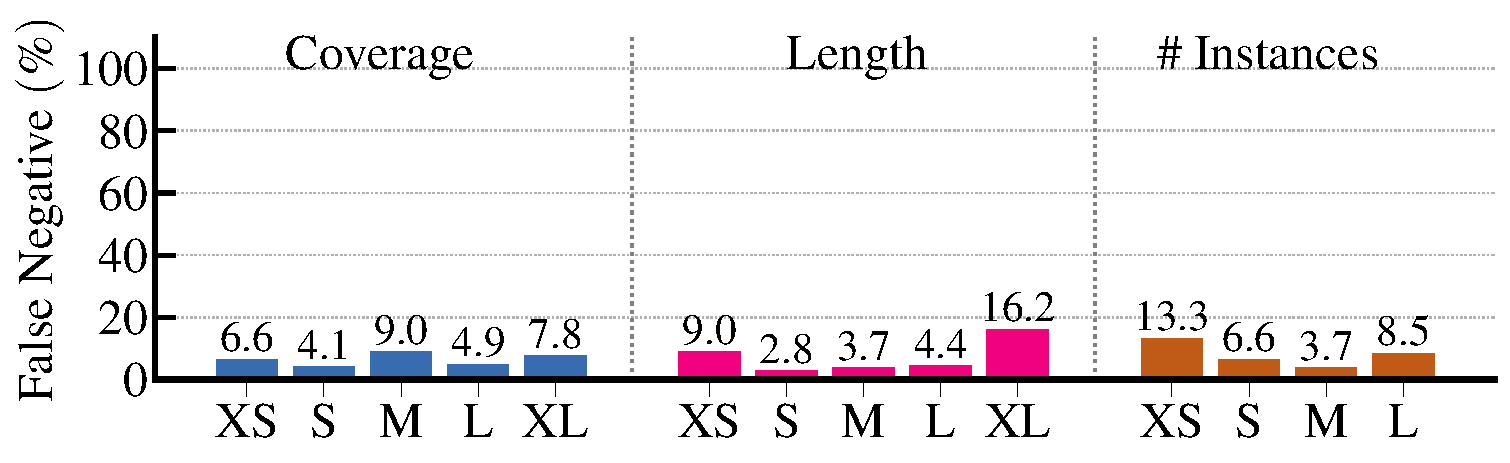
\includegraphics[width=0.6\linewidth]{sup_figures/false_negative_analysis.pdf}
      \caption{False negative (FN) profiling of our results on THUMOS14 using~\cite{detadeccv2018}. This figure shows the FN rates under different video contents. From this figure we can find that our model will suffer from extra short or extra long instances. Also, our model will suffer from video inputs which have a large number of action instances.}\label{fig:false negative}
\end{figure*}
\begin{figure*}[th!]
    \centering
    
\includegraphics[width=0.75\linewidth]{sup_figures/sensitivity_analysis.pdf}
    \caption{Sensitive analysis of our results on THUMOS14 using~\cite{detadeccv2018}. \emph{Left}: normalized mAP at tIoU$=$0.5 under different video contents. \emph{Right}: The relative normalized mAP change at tIoU$=$0.5 with respect to different characteristics of the ground truth instances.}
    \label{fig:sensitive analysis}
\end{figure*}
\begin{figure*}[th!]
    \centering
    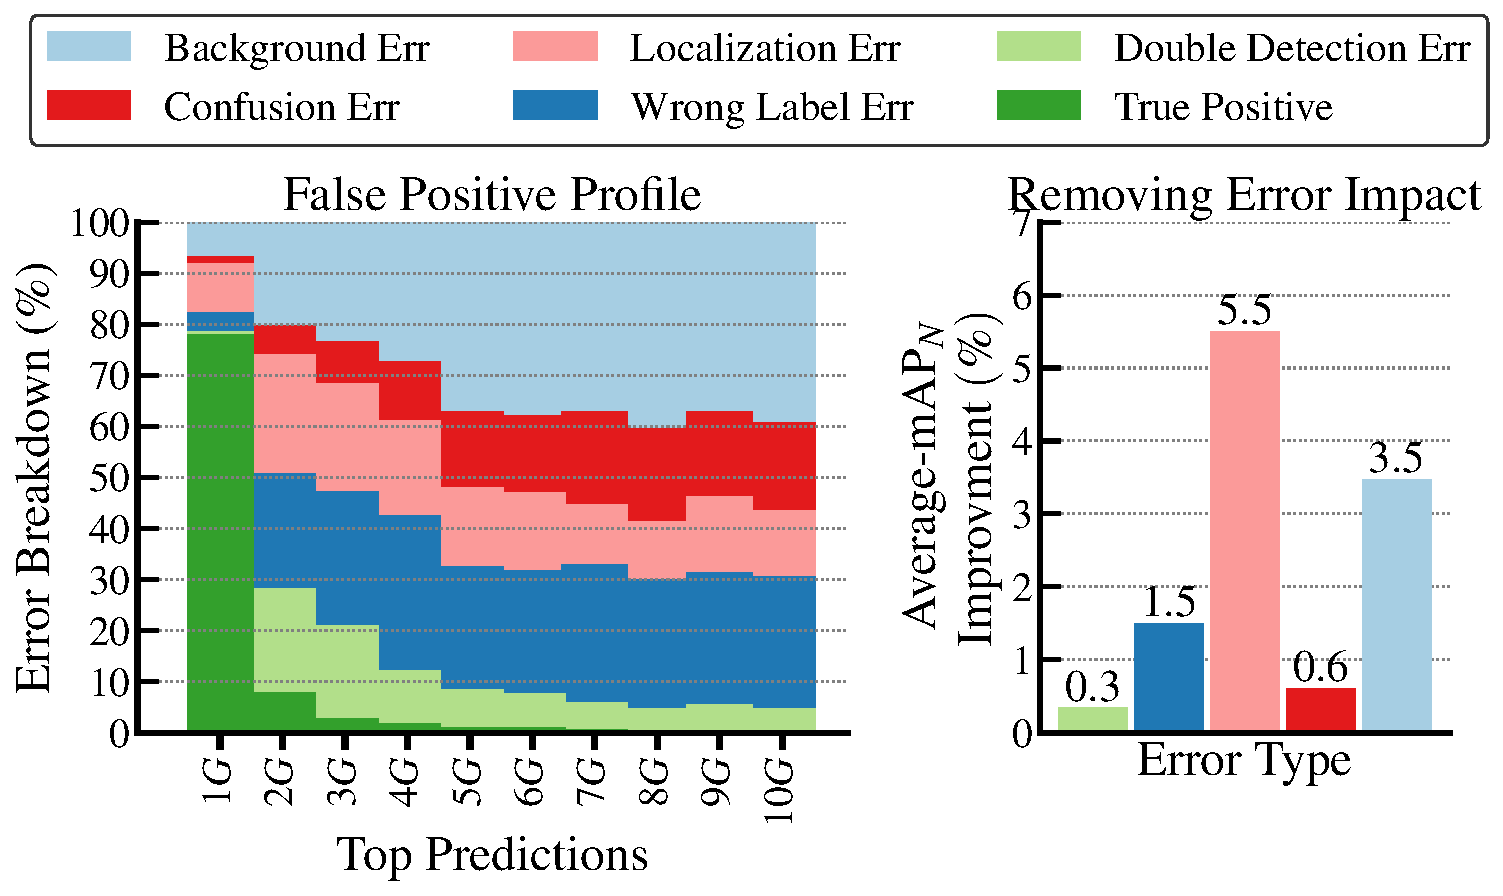
\includegraphics[width=0.9\linewidth]{sup_figures/false_positive_analysis.pdf}
    \caption{False positive (FP) profiling of our results on THUMOS14 using~\cite{detadeccv2018}. \emph{Left}: FP error breakdown when considering the predictions for the top-10 ground-truth (G) instances. \emph{Right}: The impact of error types. Localization error and background confusion are the top two error types.}
    \label{fig:false positive}
\end{figure*}

\noindent \textbf{Metrics}. In~\cite{detadeccv2018}, several characteristic metrics were defined given a dataset (\eg THUMOS14), including coverage, length, and the number of instances. Specifically, coverage presents the relative length of the actions (compared to the whole video), categorized into five bins: Extra Small (XS: (0, 0.02]), Small (S: (0.02, 0.04]), Medium (M: (0.04, 0.06]), Large (L:(0.06, 0.08]), and Extra Large (XL: (0.08, 1.0]). Length denotes the absolute length~(in seconds) of actions, organized into five length groups: Extra Small (XS: (0, 3]), Small (S: (3, 6]), Medium (M: (6, 12]), Long (L: (12, 18]), and Extra Long (XL: $>$ 18). Moreover, number of instances refers to the total count of instances (from the same class) in a video. This number is further divided into four parts, including Extra Small (XS: 1); Small (S: [2, 40]); Medium (M: [40, 80]); Large (L: $>$ 80).\medskip 

\noindent \textbf{Results and Analyses}. Fig.\ \ref{fig:false negative} presents the false negative profiling. In Fig.\ \ref{fig:false negative}, we breakdown the false negative rates under the different coverage, length, and the number of instances. Our results have similar false negative rates across different coverage categories, yet have much higher false negative rates on action instances that are either very shot or very long (length), and on videos that contains many action instances (\#instances). These action instances and videos are naturally more challenging. 

Fig.\ \ref{fig:sensitive analysis} presents the sensitivity analysis of our results, \ie, normalized mAP at tIoU$=$0.5 under different characteristic metrics (left) and the variance of mAP across categories (right). Our model performs better on simple context scenarios, including XS/S/M/L coverage, S/M length and XS \#instances, and worse on more complicated scenarios. The trend is similar to the false negative profiling in Fig.\ \ref{fig:false negative}. Moreover, our model is robust across different categories in coverage, length and \#instances with small variances. 

\section{Implementation Details}\label{sec:appendix:details}
We now present implementation details including the network architecture, training and inference. Further details can be found in our code.

\begin{table*}[t!]
	\centering
	\caption{\textbf{The architecture of our model.} Our network consists of (1) a Transformer encoder (first row block) and (2) a lightweight convolutional decoder with the classification / regression heads (last row block). For each layer, we list the layer name, layer parameters, the input to the layer, and the output feature size. We also include its regression range (in seconds for THUMOS14 and EPIC-Kitchens 100 and in number of time steps for ActivityNet-1.3). For convolutional layers, $k$ is the kernel size of 1D convolutions and $s$ is the stride, and $c_{i},c_{o}$ is the input and output feature channel, respectively. For Transformer Unit, $ds$ is the downsampling ratio. $T$ is the temporal length of input sequence and $D$ is the input feature dimension. For classification head, the output dimension is the number of action categories. For regression head, the output dimension is 2, \ie, distances to action onset and offset.}
    \resizebox{1.0\textwidth}{!}{
	\begin{tabular}{c|c|c|c|c|c}
	    &
		\multicolumn{1}{c|}{Name} & 
		\multicolumn{1}{c|}{Layer} & 
		\multicolumn{1}{c|}{Input} & \multicolumn{1}{c|}{\begin{tabular}[c]{@{}c@{}}Output Size\\ (T $\times$ D)\end{tabular}} & 
		\multicolumn{1}{c}{\begin{tabular}[c]{@{}c@{}}Regression\\ Range\end{tabular}} \\
		\hline
		\multirow{13}{*}{encoder} & input clip        &  -    & - & T$\times$D    & - \\
		&projection1       &  conv $k$=3, $s$=1 ($c_{i}$ = D, $c_{o}$ = 512)  & input clip & T $\times$ 512 &-\\
		&projection2       &  conv $k$=3, $s$=1 ($c_{i}$ = 512, $c_{o}$ = 512)  & projection1 & T $\times$ 512 &-\\
		&transformer0 &  Transformer Unit, $ds$=1  & projection2 &  T $\times$ 512 & -\\
		&transformer1 &  Transformer Unit, $ds$=1  & transformer0 &  T $\times$ 512 & [0, 4)\\
		&transformer2 &  Transformer Unit, $ds$=2  & transformer1 &  T/2 $\times$512 & [4, 8) \\ 
        &transformer3 & Transformer Unit, $ds$=2   & transformer2 &  T/4 $\times$512& [8, 16)\\
        &transformer4 & Transformer Unit, $ds$=2   & transformer3 &  T/8 $\times$512& [16, 32)\\
		&transformer5 & Transformer Unit, $ds$=2   & transformer4 &  T/16 $\times$512 & [32, 64)\\
		&transformer6 & Transformer Unit, $ds$=2   & transformer5 &  T/32 $\times$512 & [64, $+\infty$)\\
		\hline
		\multirow{3}{*}{\begin{tabular}[c]{@{}c@{}}decoder\\ (heads)\end{tabular}} &\multirow{3}{*}{cls / reg nets} &  conv $k$=3, $s$=1 ($c_{i}$ = 512, $c_{o}$ = 512) &  transformer1,...,transformer6 &[T/32$\times$512,$\ldots$, T$\times$512]&-\\
		& &  conv $k$=3, $s$=1 ($c_{i}$ = 512, $c_{o}$ = 512) & transformer1,...,transformer6  & [T/32$\times$512,$\ldots$, T$\times$512]&-\\
		& &  conv $k$=3, $s$=1 ($c_{i}$ = 512, $c_{o}$ = output) & transformer1,...,transformer6 & [T/32$\times$output,$\ldots$, T$\times$output]&-\\
	\end{tabular}}
	\label{table:network structure on THUMOS14 and EPIC-Kitchens}
\end{table*}

\medskip
\noindent \textbf{Network Architecture}.
We present our network architecture in Table~\ref{table:network structure on THUMOS14 and EPIC-Kitchens}, as described in Sec.\ 3. In the ablation study (Sec.\ 4), we also considered a baseline that replaces the Transformer Units in Table~\ref{table:network structure on THUMOS14 and EPIC-Kitchens} with convolution blocks, following the design of a bottleneck block in ResNet~\cite{resnetcvpr2016}. Specifically, a stack of three 1D convolutional layers were used. The kernel size of three convolutional layers were 1, 3 and 1, respectively. The expansion factor of the bottleneck block was 2. We added an extra strided convolutional layer with kernel size=1 and stride=2 to perform downsampling when necessary. 

\medskip
\noindent \textbf{Training Details}. For training, we considered both fixed length inputs (ActivityNet) and variable length inputs (THUMOS14, ActivityNet, and EPIC-Kitchens 100). For variable length inputs, we capped the input length to 2304 (around 5 minutes on THUMOS14 and around 20 minutes on EPIC-Kitchens 100), and randomly selected a subset of consecutive clips from an input video. Position embedding was disabled by default except for ActivityNet. Model EMA~\cite{huang2017snapshot} and gradient clipping were also implemented to further stabilize the training. Hyperparameters were slightly different across datasets and discussed later in our experiment details. 

\medskip
\noindent \textbf{Inference Details}. For fixed length inputs (ActivityNet-1.3), we fed the full sequence into our model. For variable length inputs (THUMOS14 and EPIC-Kitchens 100), we sent the full sequence into the model. When using position embeddings in our ablation study, we adopted the technique from~\cite{vitarxiv2020}. Specifically, for input sequences shorter than the training sequence length (2304), we fed the full sequence into our model and clipped the position embedding using the actual length of the video. For input sequences longer than the training sequence length, we again fed the full sequence into our model, yet used linear interpolation to upsample the position embeddings.

\medskip
\noindent \textbf{Score Fusion}. For our experiments on THUMOS14 and ActivityNet-1.3, we sometimes consider score fusion using external classification scores. Specifically, given an input video, the top-2 video-level classes given by external classification scores were assigned to all detected action instances in this video, where the action scores from our model were multiplied with the external classification scores. Each detected action instance from our model thus creates two action instances. We refer the readers to~\cite{pgcniccv2019} (Appendix E) for a more detailed description of the score fusion strategy. 



\medskip
\noindent \textbf{Experiment Details}.
Our experiment details vary across datasets, as each dataset includes videos of different resolution and frame rate, and considers different types of features. We now describe our experiment details for THUMOS14, ActivityNet-1.3, and EPIC-Kitchens 100.\smallskip

\squishlist
\item \textbf{THUMOS14}: We used two-stream I3D~\cite{kinetics2017cvpr} pretrained on Kinetics to extract the video features on THUMOS14, following~\cite{cmcscvpr2019,bottumuptaleccv2020}. We fed 16 consecutive frames as the input to I3D, used a sliding window with stride 4 and extracted 1024-D features before the last fully connected layer. The two-stream features were further concatenated (2048-D) as the input to our model. \textit{m}AP@$[0.3$:$0.1$:$0.7]$ was used to evaluate our model. Our model was trained for 50 epochs with a linear warmup of 5 epochs. The initial learning rate was 1e-4 and a cosine learning rate decay is used. The mini-batch size was 2, and a weight decay of 1e-4 was used.

\item \textbf{ActivityNet-1.3}: We used two-stream I3D~\cite{kinetics2017cvpr} and TSP~\cite{tspiccvworkshop2021} for feature extraction, and increased the stride of the sliding window to 16. Following \cite{bsneccv2018,bmniccv2019,gtadcvpr2020}, the extracted features were downsampled into a fixed length of 160 and 192 using linear interpolation for I3D and TSP features, respectively. For evaluation, we used \textit{m}AP@$[0.5$:$0.05$:$0.95]$ and also reported the average \textit{m}AP. Our model was trained for 15 epochs with a linear warmup of 5 epochs. The learning rate was 1e-3, the mini-batch size was 16, and the weight decay was 1e-4. For ActivityNet, we find it is helpful to train our model to generate proposals by considering all actions from a single category, and then use external classification scores for the recognition. This strategy was also used in previous single-stage TAL methods~\cite{afsdcvpr2021}. 

\item \textbf{EPIC-Kitchens 100}: We used a SlowFast network~\cite{slowfasticcv2019} pre-trained on EPIC-Kitchens for feature extraction. This model is provided by~\cite{epicarxiv2020}. We fed 32 frame window with a stride of 16 to extract 2304-D features. Our model was trained on the training set and evaluated on the validation set. A window size of 9 was used for local self-attention. For evaluation, we used \textit{m}AP@$[0.1$:$0.1$:$0.5]$ and report the average \textit{m}AP following~\cite{epicarxiv2020}. Our model was trained for 30 epochs with learning rate 1e-4, mini-batch size 2, and weight decay of 1e-4. 
\squishend

\begin{figure*}[t]
\begin{center}
    \minipage{0.48\textwidth}
      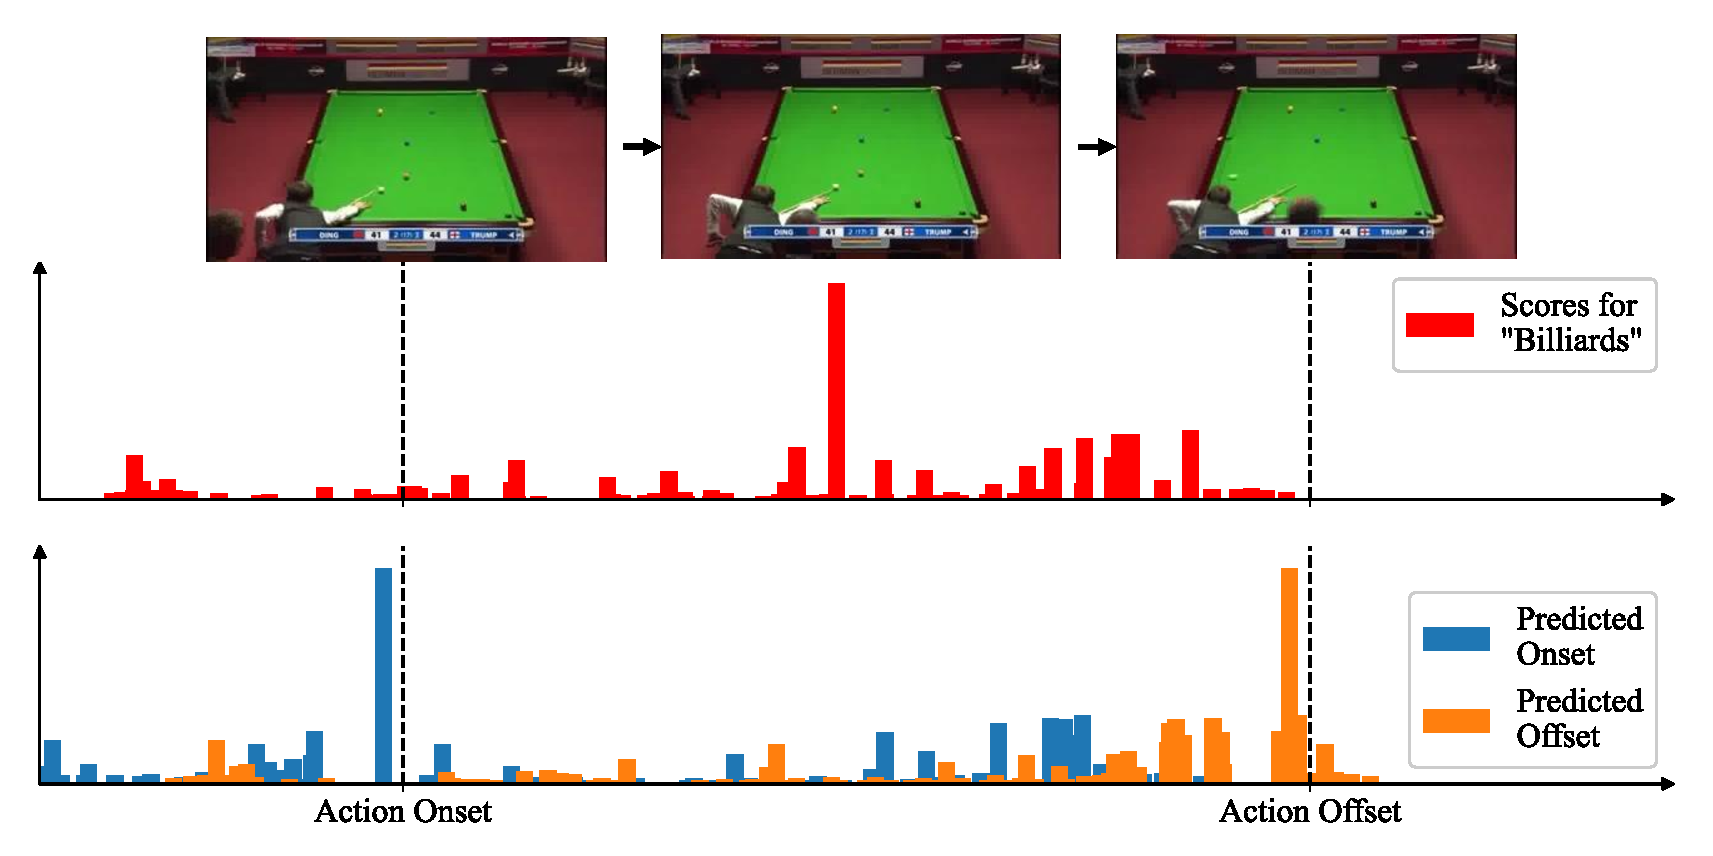
\includegraphics[width=\linewidth]{sup_figures/Vis4-new.pdf}
    \endminipage\hfill
    \minipage{0.48\textwidth}%
      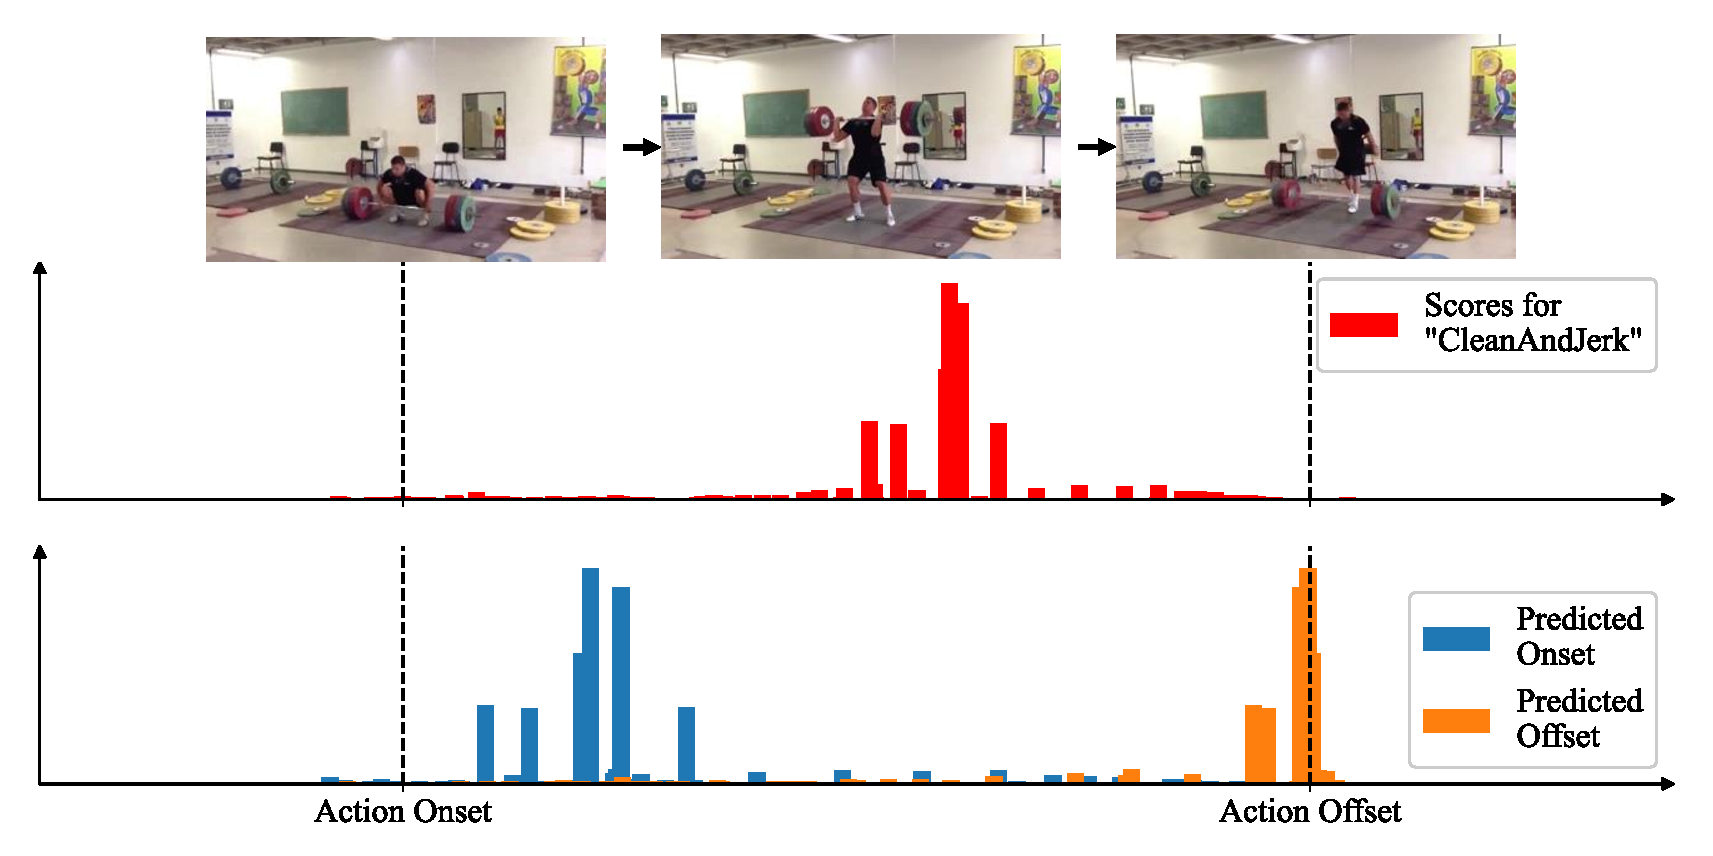
\includegraphics[width=\linewidth]{sup_figures/Vis7-new.pdf}
    \endminipage \\
    \minipage{0.48\textwidth}
      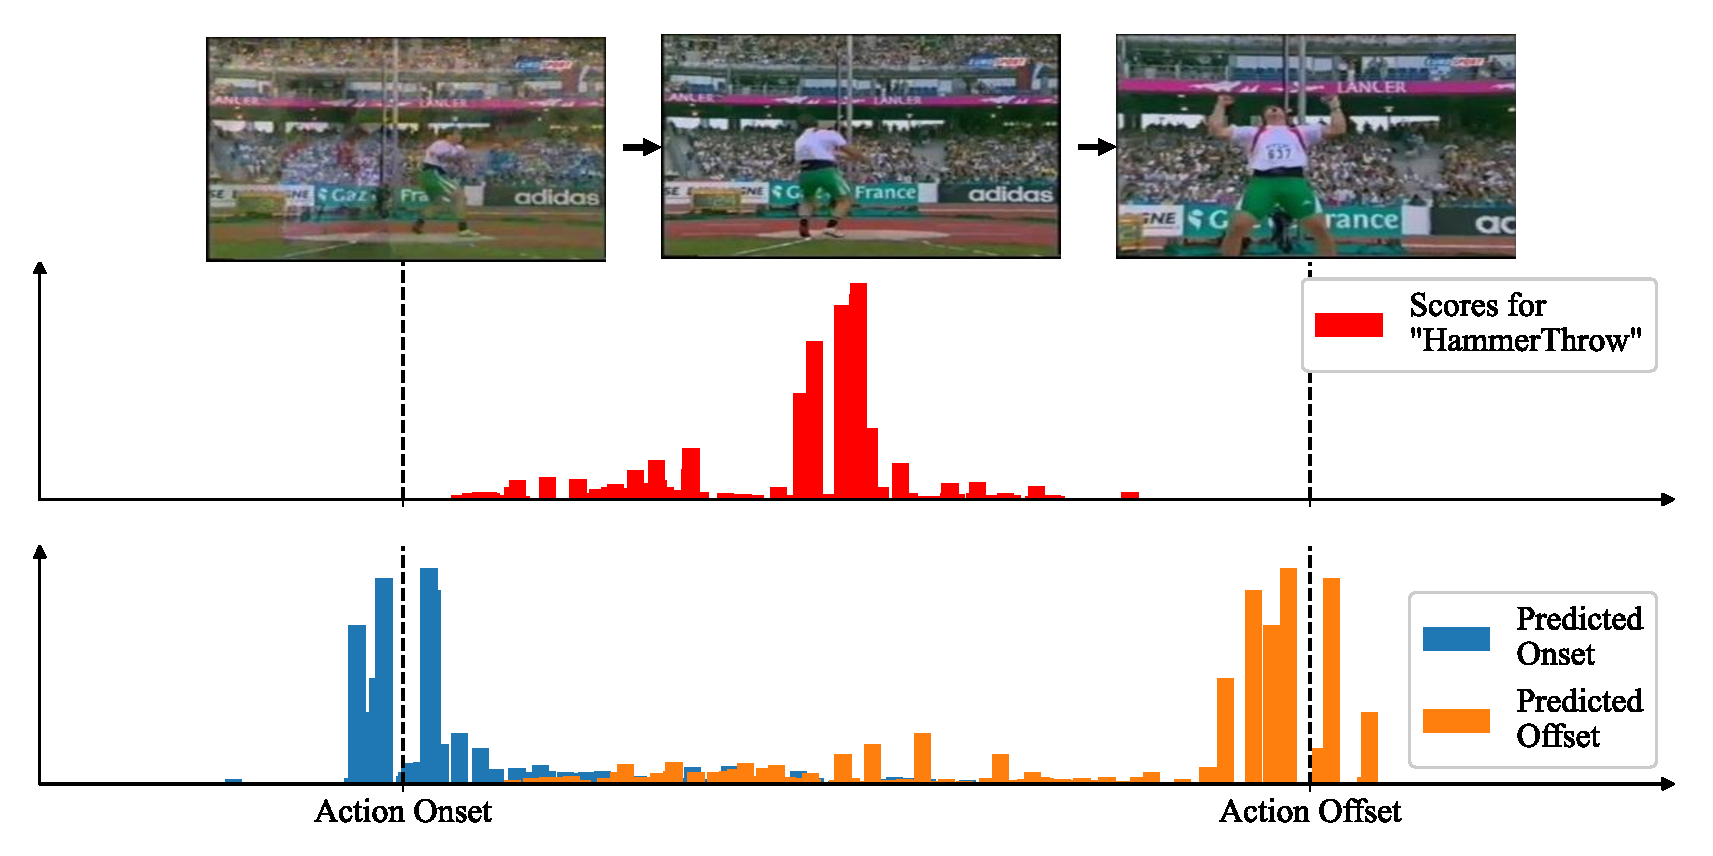
\includegraphics[width=\linewidth]{sup_figures/Vis5-new.pdf}
    \endminipage\hfill
    \minipage{0.48\textwidth}%
      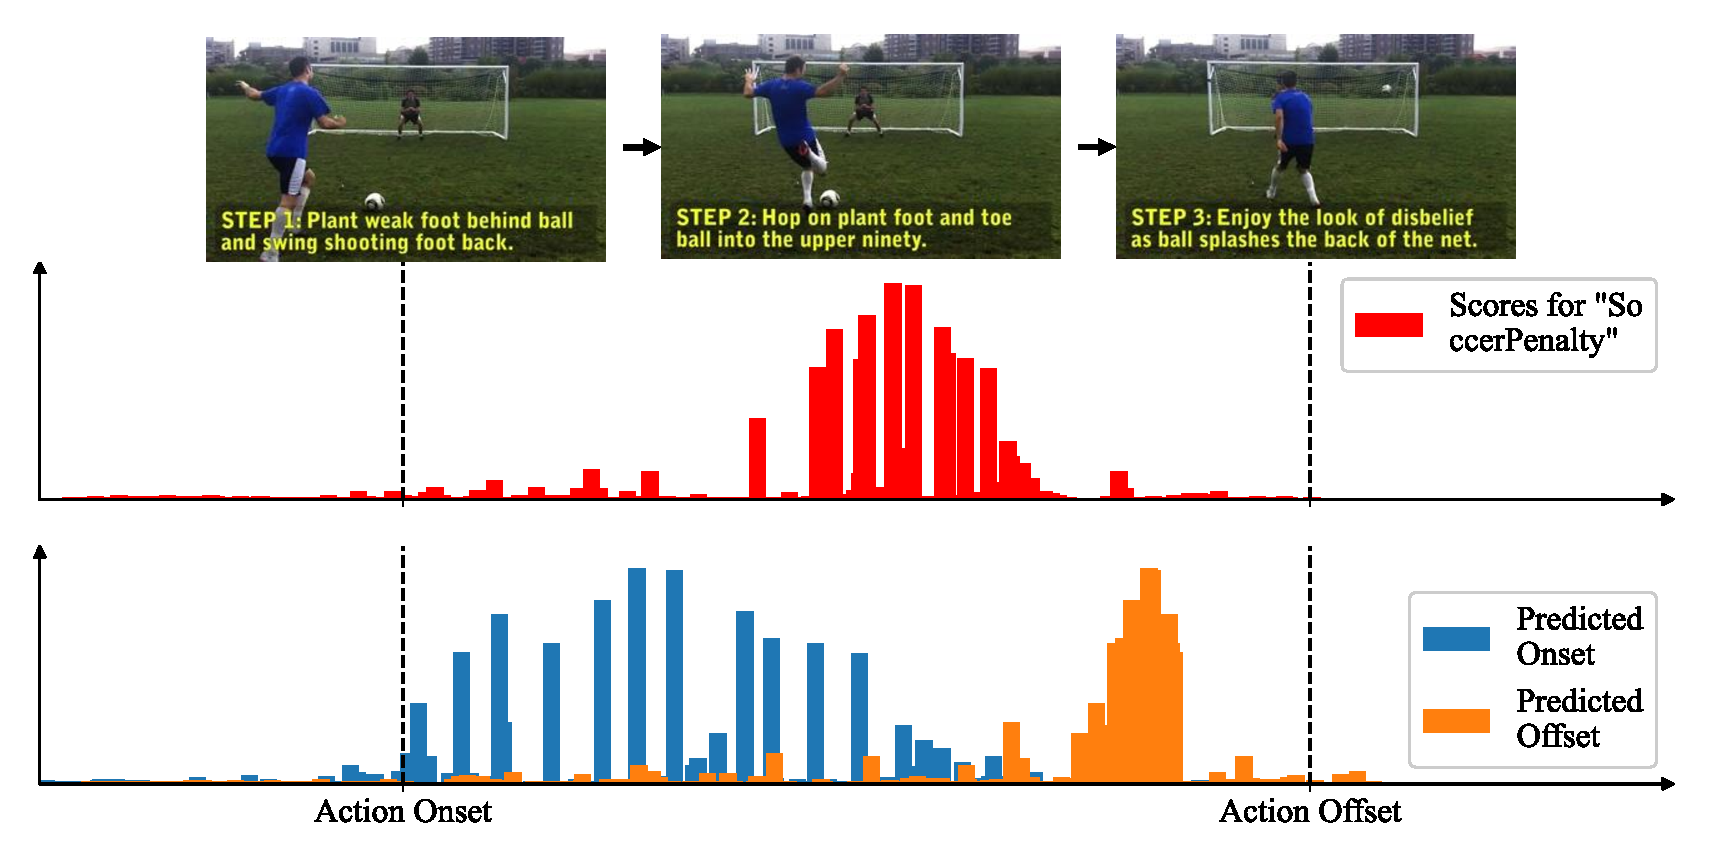
\includegraphics[width=\linewidth]{sup_figures/Vis8-new.pdf}
    \endminipage\\
    \minipage{0.48\textwidth}
      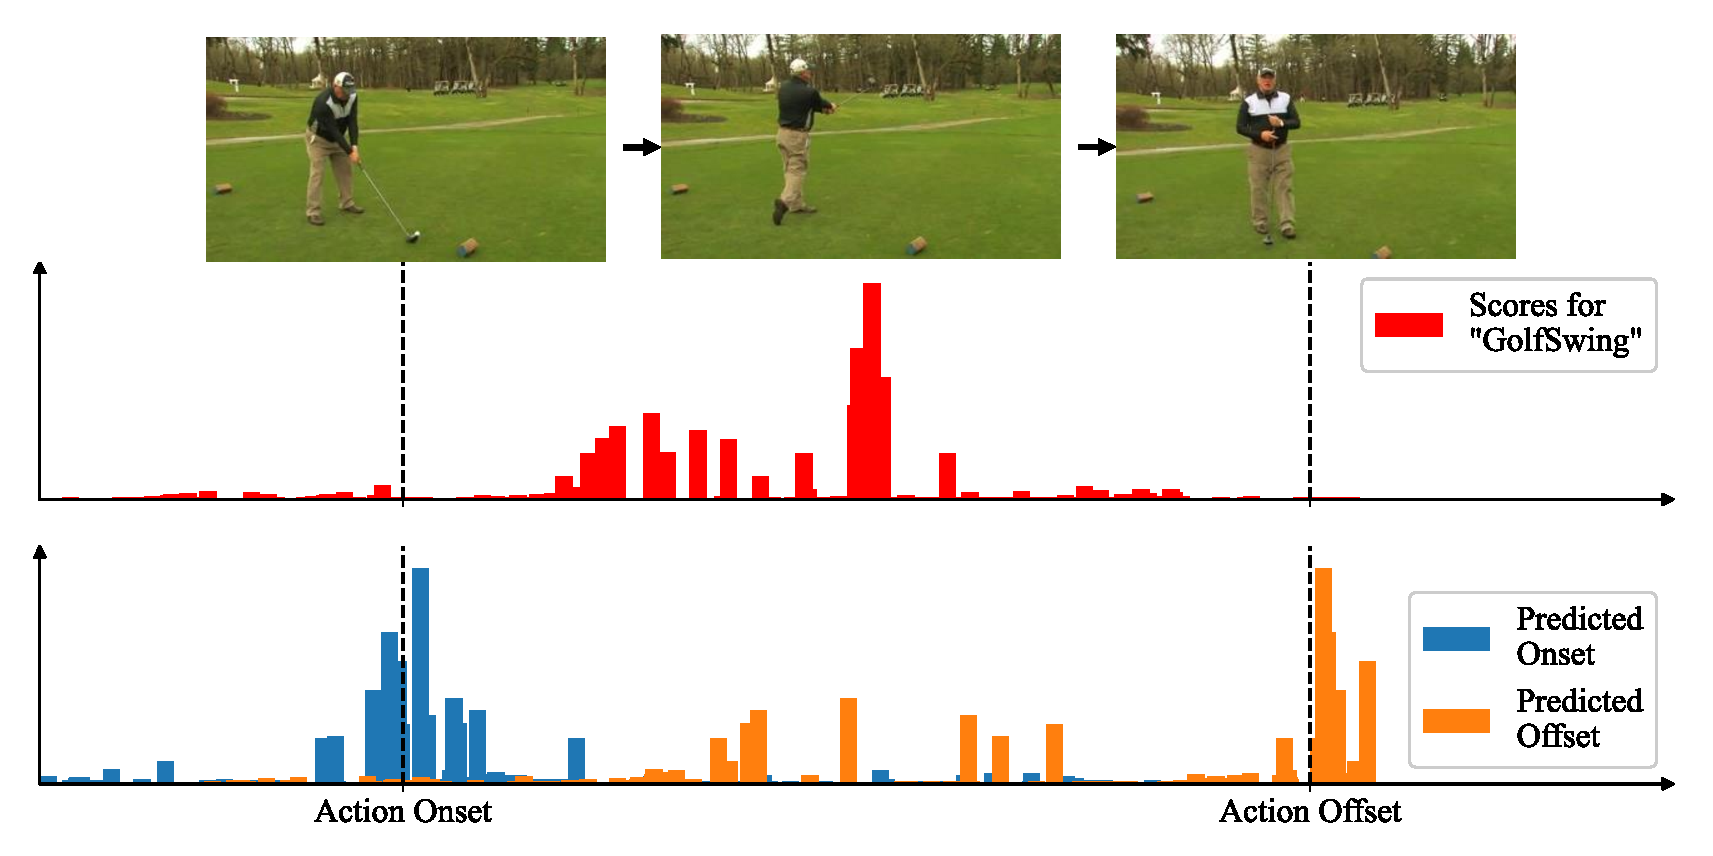
\includegraphics[width=\linewidth]{sup_figures/Vis6-new.pdf}
    \endminipage\hfill
    \minipage{0.48\textwidth}%
      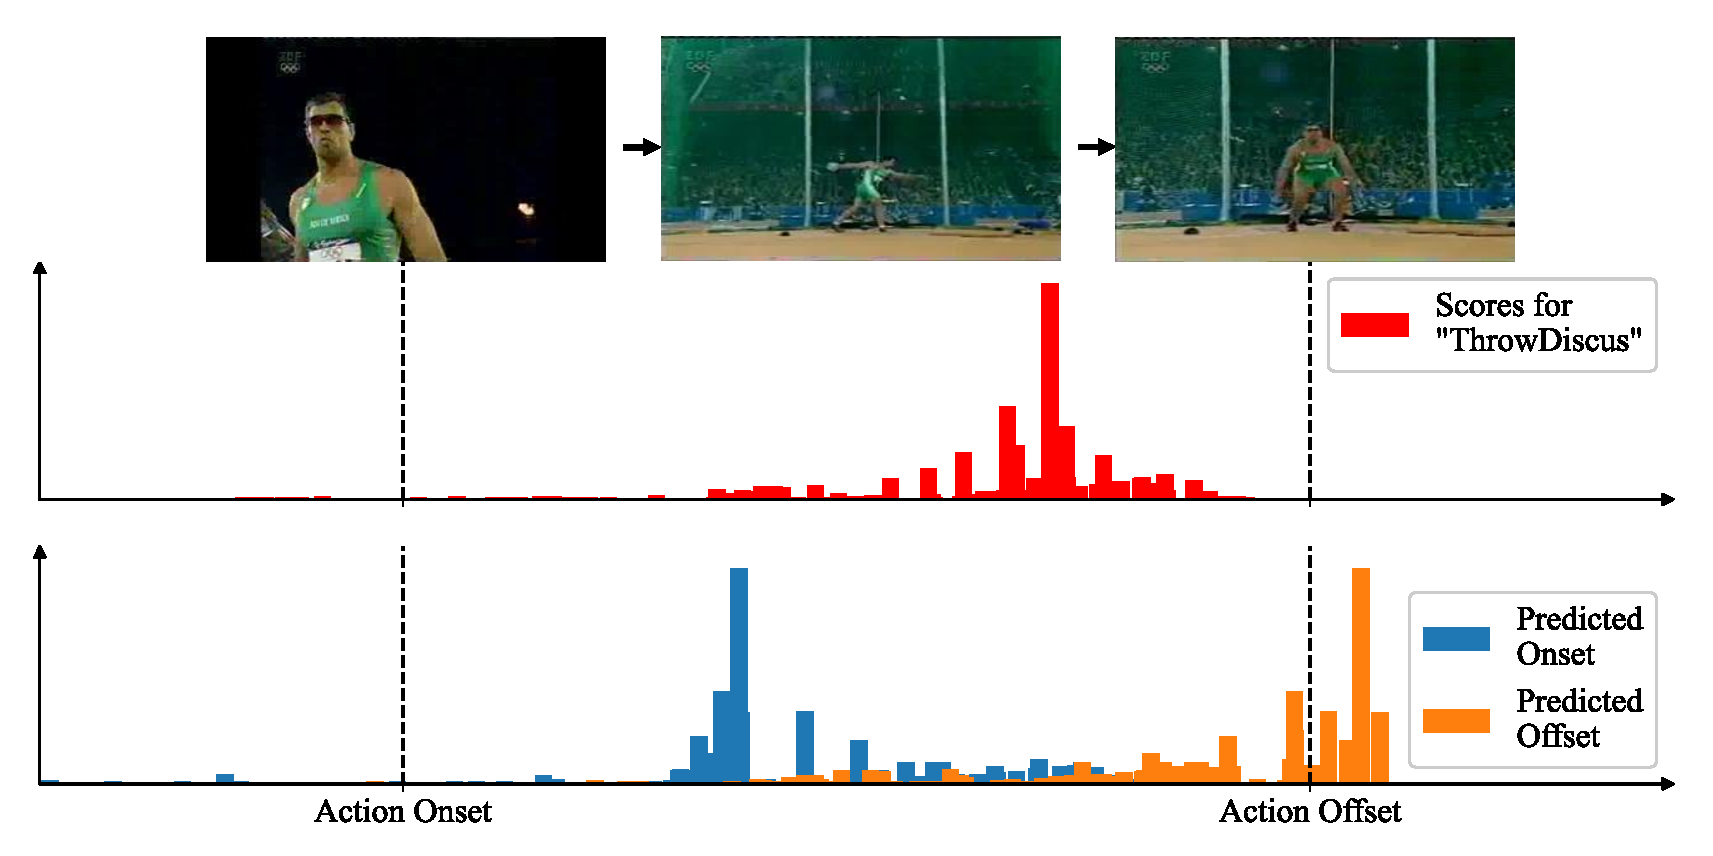
\includegraphics[width=\linewidth]{sup_figures/Vis9-new.pdf}
    \endminipage
\end{center}
\caption{More visualization of our outputs. For each item from \emph{top} to \emph{bottom}: (1) the input video frames;  (2) action scores at each time step; (3) histogram of action onsets and offsets computed by weighting the regression outputs using the action scores. \emph{Left}: successful cases; \emph{Right}: failure cases. This figure is best viewed in color and when zoomed in.}
\label{fig:more vis}
\end{figure*}

\medskip
\noindent \textbf{Reproducibility of Our Results}. All results reported in the paper were obtained with the same random seed using PyTorch 1.10, CUDA 10.2 and CUDNN 7.6.5 on an NVIDIA Titan Xp GPU, using deterministic GPU computing routines. On the same machine, our code will always produce the same results when using the same random seed. Across machines/GPUs and computing environments, we have observed minor variation of average mAP scores (up to 0.5\% average mAP on THUMOS, less than 0.2\% average mAP on ActivityNet, and under 0.8\% average mAP on EPIC Kitchens), yet those minor variations do not erode the clear performance gains of our method. Our code is made publicly available.\medskip

\section{Additional Visualizations}\label{sec:appendix:vis}
Further, we present more visualizations of our results in Fig.\ \ref{fig:more vis}, extending Fig.\ 3 of the main paper. Our model is able to detect the occurrence of actions and estimate their temporal boundaries for the most of the cases (see the first column of Fig.\ \ref{fig:more vis}). The major failure modes of our model, as demonstrated in the second column of Fig.\ \ref{fig:more vis}, include (1) incorrect classification of action centers, \ie background confusion (classification errors); (2) inaccurate regression of the action's onset and offset (localization errors). We plan to address these issues in our future work.

\section{Limitations and Future Work}\label{sec:appendix:limit}
A main limitation of our method is the use of pre-extracted video features, also faced by many previous approaches. Another limitation is the need for many human labeled videos for training and the constraint of a pre-defined vocabulary of actions. Interesting future directions include pre-training for action localization~\cite{tspiccvworkshop2021,xu2021boundary}, and learning from videos and text corpus~\cite{radford2021learning,jia2021scaling} without human labels.

